En esta sección se presentan los resultados obtenidos tras la implementación del sistema blockchain para el almacenamiento inmutable de logs de seguridad. Los resultados demuestran el cumplimiento exitoso de los objetivos específicos planteados, evidenciando la funcionalidad completa del sistema desarrollado mediante capturas de pantalla, consultas directas a la blockchain y métricas de rendimiento del sistema implementado.

\subsection{Levantamiento de la Red Blockchain}
La demostración práctica del sistema que aquí se está desarrollando comienza con el levantado de la infraestructura blockchain. Ello es la base fundamental donde se ejecutará todo el sistema de gestión de logs de seguridad, por lo que ha sido completamente automatizado para garantizar consistencia y minimizar errores de configuración manual.
Para facilitar el despliegue y reducir la complejidad operacional, se implementó un script de inicialización que coordina el levantamiento de todos los componentes de la red Hyperledger Fabric. Como se muestra en la Fig \ref{fig:script_inicio}, el comando de ejecución es directo y simple:
\begin{figure}[htbp]
    \centering
    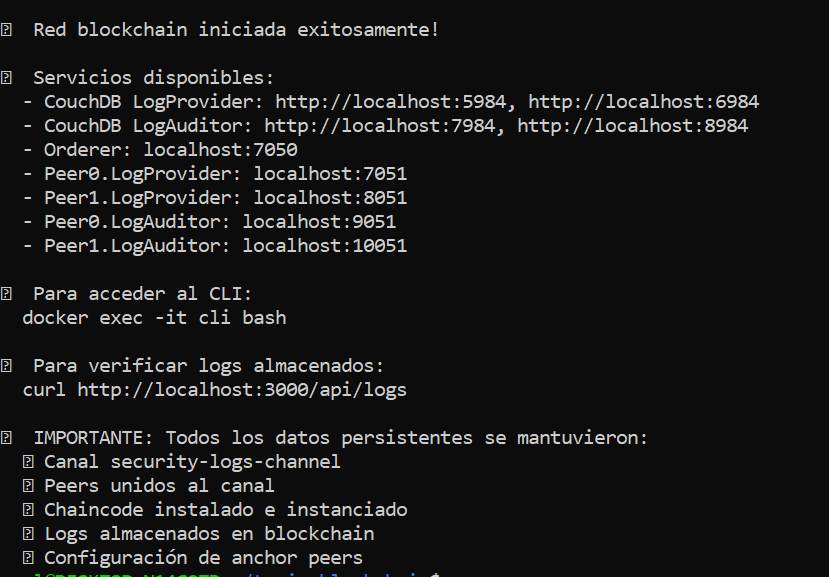
\includegraphics[width=0.8\textwidth]{figuras/script_inicio.png}
    \caption{Ejecución del script de inicialización de la red blockchain}
    \label{fig:script_inicio}
\end{figure}

El script ejecuta una secuencia predefinida de pasos que aseguran la correcta inicialización de cada componente. Esta automatización resultó esencial durante las múltiples iteraciones de prueba del sistema, ya que permite recrear el entorno completo en cuestión de minutos.

\subsection{Verificación de Componentes Activos}
Una vez completado el proceso de inicialización, es crucial verificar que todos los servicios estén operativos. La Fig \ref{fig:docker_ps} muestra el resultado del comando de verificación.
\begin{figure}[H]
    \centering
    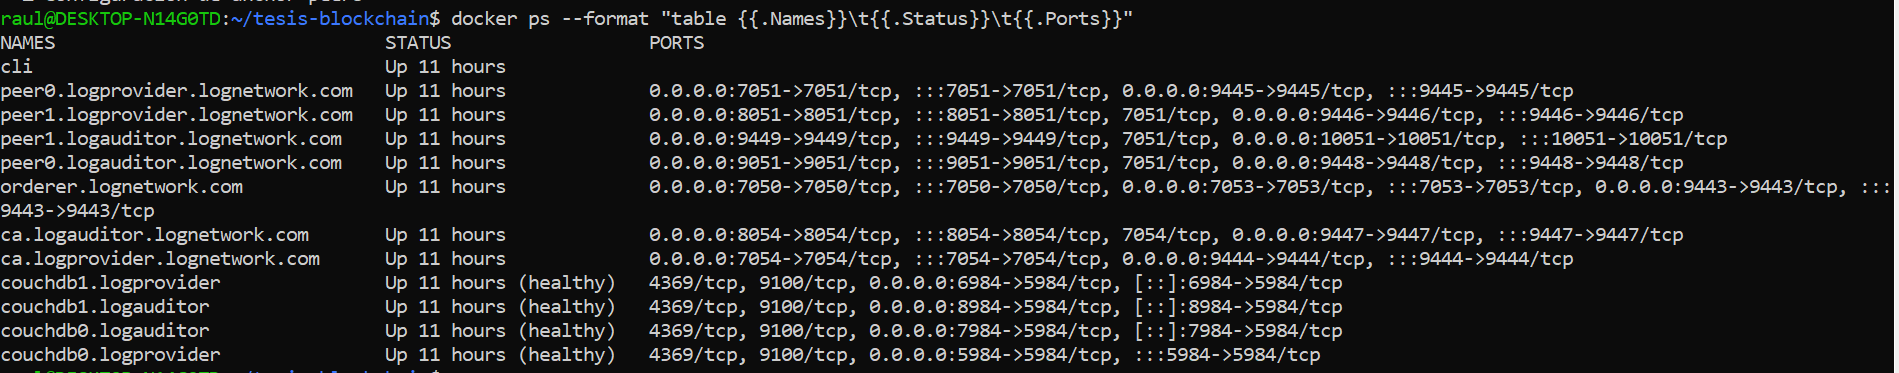
\includegraphics[width=0.9\textwidth]{figuras/docker_ps.png}
    \caption{Contenedores Activos de la Red Blockchain}
    \label{fig:docker_ps}
\end{figure}

Esta verificación confirma que los ocho contenedores principales están ejecutándose correctamente: cuatro nodos peer (dos por organización), un orderer, un CLI, y las instancias de CouchDB correspondientes. El estado “Up” indica que los servicios han superado sus verificaciones de salud internas.

\subsection{Validación del Canal de Comunicación}
Con la infraestructura desplegada, se verifica que el canal security-logs-channel ha sido creado exitosamente. Este canal constituye el espacio compartido donde ambas organizaciones interactúan para el almacenamiento y consulta de logs de seguridad:

Como se observa en la Fig \ref{fig:canal_creado}, el comando \textit{peer channel list} muestra que el canal security-logs-channel está disponible y operativo. Esta confirmación es fundamental ya que establece las políticas de endorsement que requieren la participación de ambas organizaciones para validar cualquier transacción de almacenamiento de logs.
\begin{figure}[H]
    \centering
    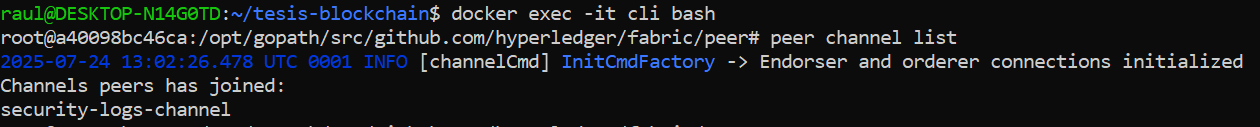
\includegraphics[width=0.8\textwidth]{figuras/canal_creado.png}
    \caption{Verificación de Participación del Peer en el Canal de Seguridad}
    \label{fig:canal_creado}
\end{figure}

\subsection{Captura Automática de Logs del Sistema}
Una vez establecida la infraestructura blockchain, el siguiente componente crítico del sistema es el mecanismo de captura automática de logs de seguridad. Este componente implementa la funcionalidad de interceptar eventos del sistema en tiempo real y determinar cuáles requieren almacenamiento inmutable en la blockchain.
\subsubsection{Inicialización del Collector de Logs}
El sistema de captura se implementó mediante un collector especializado que opera como un servidor UDP, interceptando los logs que el sistema operativo envía a través del protocolo syslog estándar. La inicialización del collector se realiza ejecutando: \textit{node syslog-collector.js}
\begin{figure}[H]
    \centering
    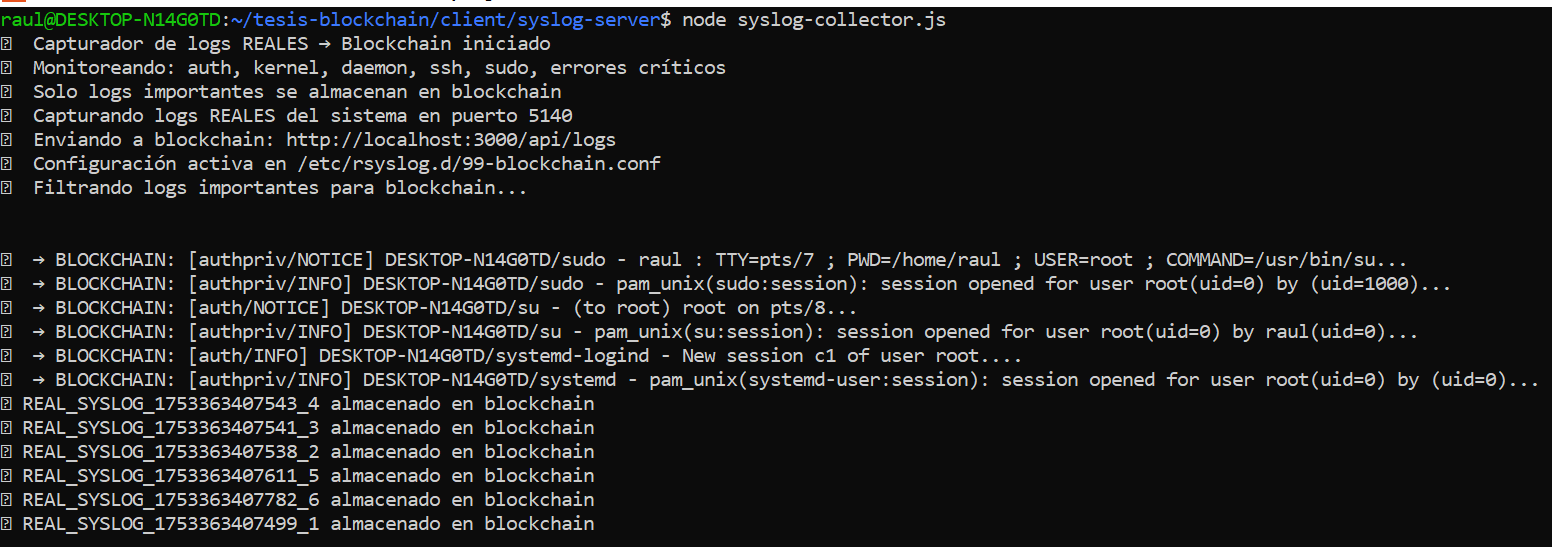
\includegraphics[width=0.8\textwidth]{figuras/collector_inicio.png}
    \caption{Ejecución del Colector de Logs y Almacenamiento en la Blockchain}
    \label{fig:collector_inicio}
\end{figure}

Como se muestra en la Fig \ref{fig:collector_inicio}, el sistema confirma la inicialización exitosa del servidor en el puerto 5140, estableciendo la conectividad con la API blockchain y activando los filtros de logs críticos. Esta configuración permite que el collector reciba automáticamente todos los eventos de seguridad generados por el sistema operativo y las aplicaciones.

\subsubsection{Prueba de Captura Manual}
Para demostrar la capacidad de respuesta del sistema, se ejecutó una prueba de generación manual de logs críticos utilizando la herramienta logger del sistema: \textit{logger -p auth.warning 
“PRUEBA: Intento de acceso no autorizado desde IP 192.168.1.200”}

Como se documenta en la Fig \ref{fig:prueba_manual}, el sistema detecta inmediatamente este evento, lo clasifica como log crítico de seguridad y procede a enviarlo automáticamente a la blockchain. La respuesta es prácticamente instantánea, demostrando la efectividad del mecanismo de captura en tiempo real.
\begin{figure}[H]
    \centering
    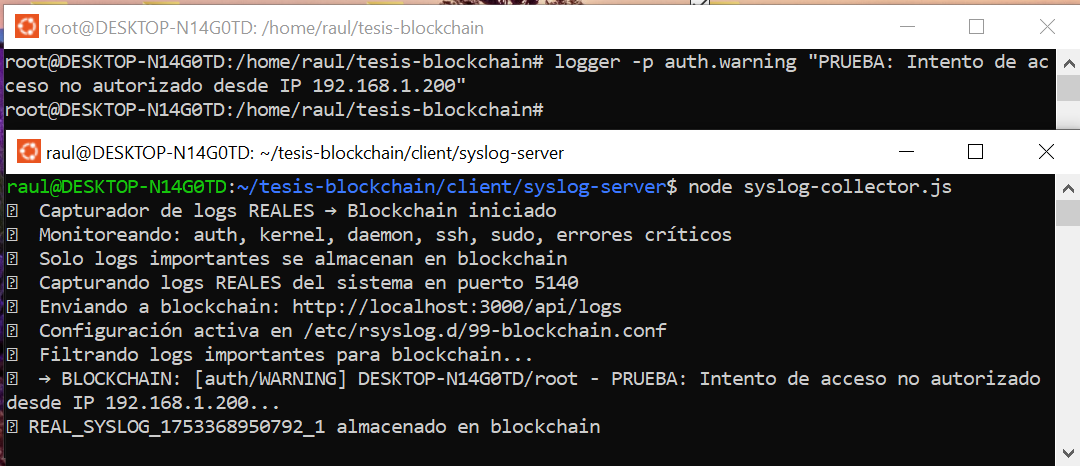
\includegraphics[width=0.8\textwidth]{figuras/prueba_manual.png}
    \caption{Prueba manual de ingreso del log}
    \label{fig:prueba_manual}
\end{figure}

Cada log que cumple los criterios de filtrado se envía automáticamente a la API REST que gestiona la interfaz con la blockchain. El collector confirma la recepción exitosa de cada log, como se muestra en la Fig \ref{fig:confirmacion_envio}, donde se puede observar el identificador único asignado y la confirmación de almacenamiento.
Esta confirmación bidireccional asegura que no se pierdan logs críticos y proporciona trazabilidad completa del proceso de captura y almacenamiento.

\begin{figure}[H]
    \centering
    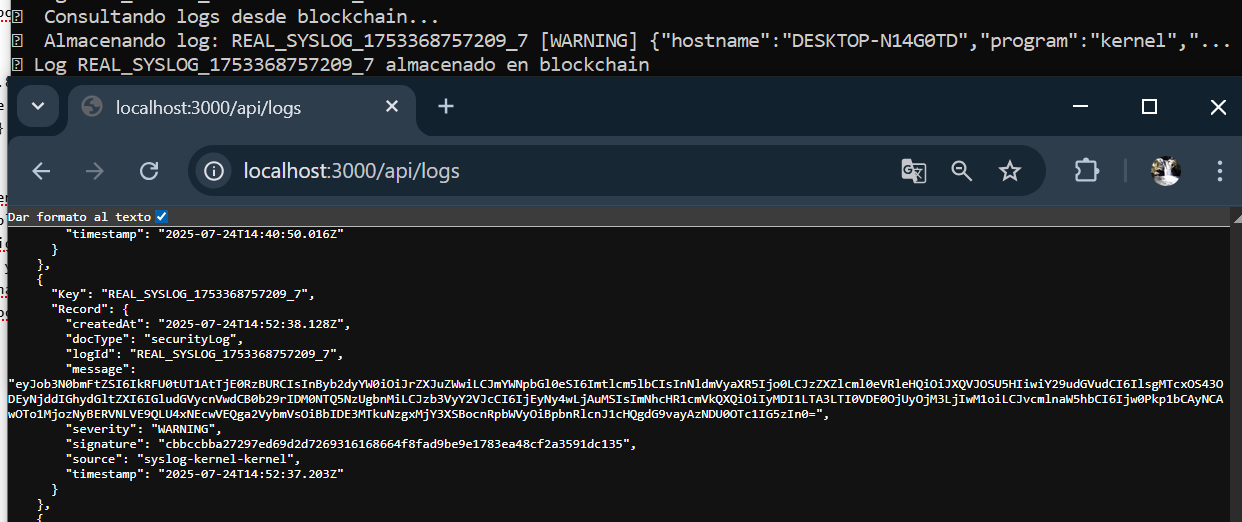
\includegraphics[width=1\textwidth]{figuras/confirmacion_envio.png}
    \caption{Confirmación de envío}
    \label{fig:confirmacion_envio}
\end{figure}

\subsection{Consulta y Verificación de Logs en Blockchain}
La fase final de la demostración del sistema consiste en verificar que los logs capturados y almacenados están efectivamente disponibles en la blockchain y pueden ser consultados a través de múltiples interfaces. Esta verificación confirma la integridad del flujo completo y demuestra las capacidades de auditoría del sistema implementado.
\subsubsection{Verificación Directa via Blockchain}
La forma más directa de verificar el almacenamiento exitoso de logs es consultando directamente la blockchain mediante el CLI de Fabric. Desde el contenedor CLI, se ejecuta \textit{peer chaincode query -C security-logs-channel -n security-logs -c '{“function”:“QuerySecurityLog”,-\\“Args”:[“REAL\_SYSLOG\_1753368757209\_7”]}'}
\begin{figure}[H]
    \centering
    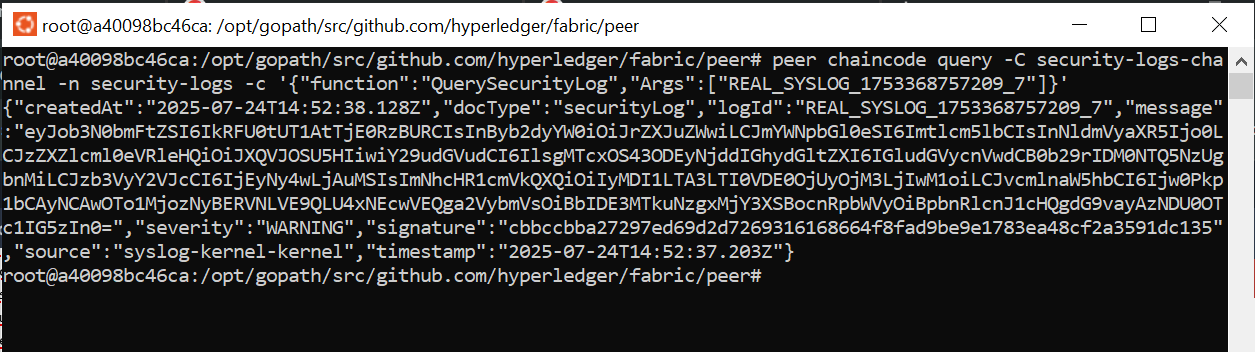
\includegraphics[width=1\textwidth]{figuras/query_blockchain.png}
    \caption{Query dentro de la blockchain}
    \label{fig:query_blockchain}
\end{figure}

Como se muestra en la Fig \ref{fig:query_blockchain}, este comando retorna todos los logs almacenados en formato JSON, incluyendo sus metadatos completos: identificadores únicos, timestamps, niveles de severidad, contenido codificado y firmas hash. Esta consulta directa confirma que los datos están efectivamente persistidos en el ledger distribuido.

\subsubsection{Consulta via API REST}
El sistema también permite la consulta de logs a través de la API REST, proporcionando una interfaz más accesible para aplicaciones externas. La consulta se realiza mediante:\textit{http://localhost:3000/api/logs}
\newpage
\begin{figure}[H]
    \centering
    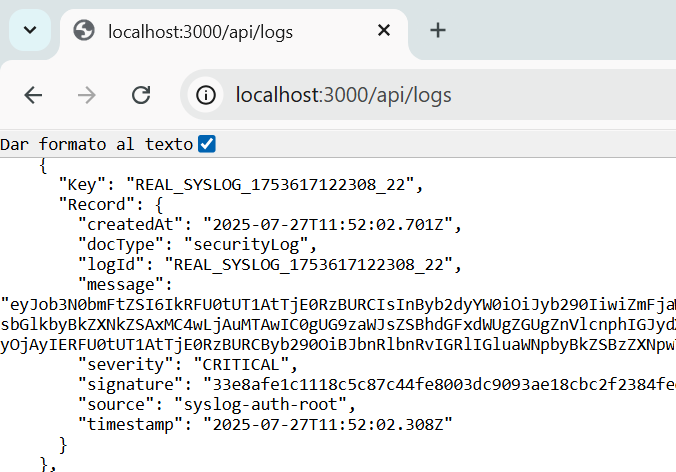
\includegraphics[width=0.8\textwidth]{figuras/api_query.png}
    \caption{Api query para la consulta de logs}
    \label{fig:api_query}
\end{figure}

La Fig \ref{fig:api_query} presenta la respuesta estructurada de la API, que incluye estadísticas del sistema como el conteo total de logs, versión del chaincode activo y timestamp de la consulta. Esta interfaz facilita la integración con sistemas de monitoreo externos y herramientas de análisis forense.


\subsubsection{Dashboard Web Interactivo}
La interfaz web desarrollada proporciona una herramienta integral para la consulta y análisis de logs de seguridad almacenados en blockchain. El dashboard implementa una consulta automáticamente a la red blockchain y presenta la información mediante visualizaciones interactivas.
Como se observa en la Fig \ref{fig:dashboard_principal}, la interfaz se estructura en componentes clave que facilitan el monitoreo de seguridad: un panel de estadísticas en tiempo real que muestra métricas esenciales del sistema , una sección dedicada al último log registrado con información completa del evento más reciente, y gráficos estadísticos que visualizan la distribución por severidad y patrones de actividad temporal.
El sistema incluye funcionalidades adicionales como visualización de logs recientes con capacidad de expansión para análisis detallado, controles de actualización automática, e indicadores de estado de conectividad. 
Esta solución demuestra la viabilidad de integrar tecnología blockchain con interfaces de usuario modernas para crear sistemas de auditoría de seguridad que combinan la inmutabilidad de los datos distribuidos con herramientas de análisis accesibles y funcionales para administradores de sistemas.
\begin{figure}[H]
    \centering
    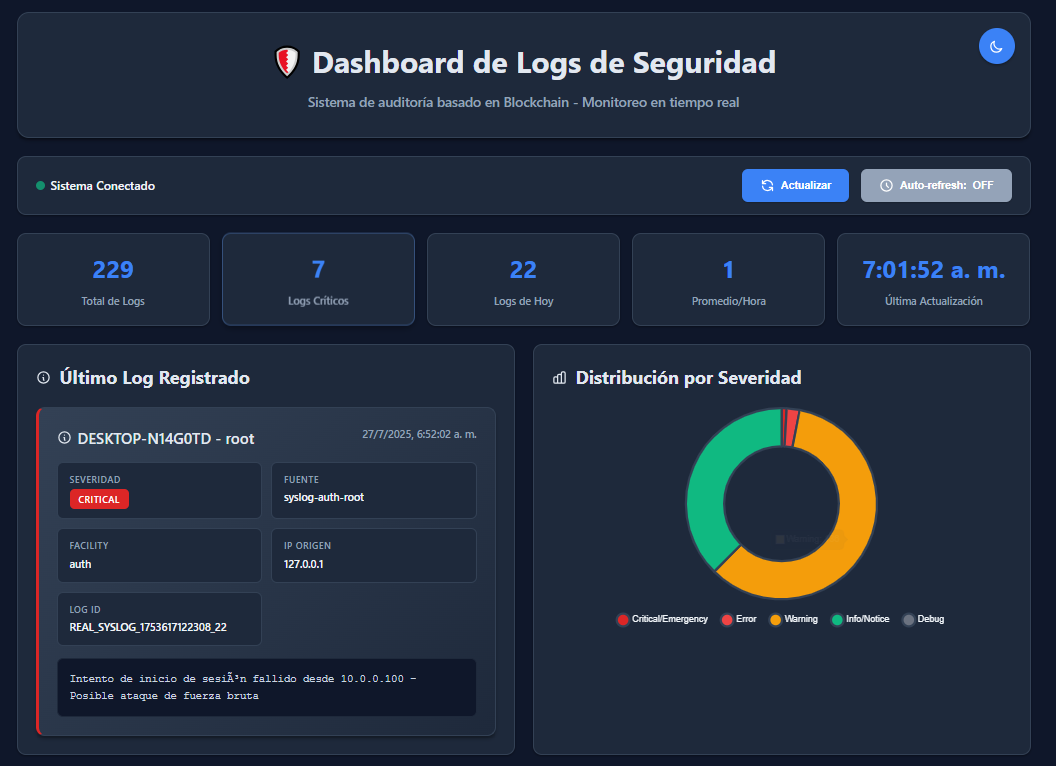
\includegraphics[width=0.8\textwidth]{figuras/dashboard_web.png}
    \caption{Dashboard principal}
    \label{fig:dashboard_principal}
\end{figure}

\subsection{Prueba de inmutabilidad}
Para demostrar la inmutabilidad de los logs de seguridad almacenados en la red blockchain basada en Hyperledger Fabric, se diseñó una prueba práctica que verifica que los logs, una vez registrados, no pueden ser modificados ni eliminados del historial de transacciones. La prueba se realizó en el canal \textit{security-logs-channel}, utilizando el chaincode \textit{security-logs}.

% Creación del log
Primero, se generó un log de seguridad mediante el comando logger, que simuló un evento de seguridad. Este log se almacenó en el ledger utilizando la función \textit{StoreSecurityLog} del chaincode. Para verificar su correcta creación, se consultó el log con el siguiente comando \textit{peer chaincode query -C security-logs-channel -n security-logs -c '{“Args”:[“QuerySecurityLog”,\\“REAL\_SYSLOG\_1753629240230\_92”]}'}

El resultado mostró los detalles del log, incluyendo su logId, timestamp, source, severity, y message, confirmando su almacenamiento en el world state (base de datos CouchDB). La salida de esta consulta se presenta en la Figura~\ref{fig:log-consultado}.

\begin{figure}[H]
    \centering
    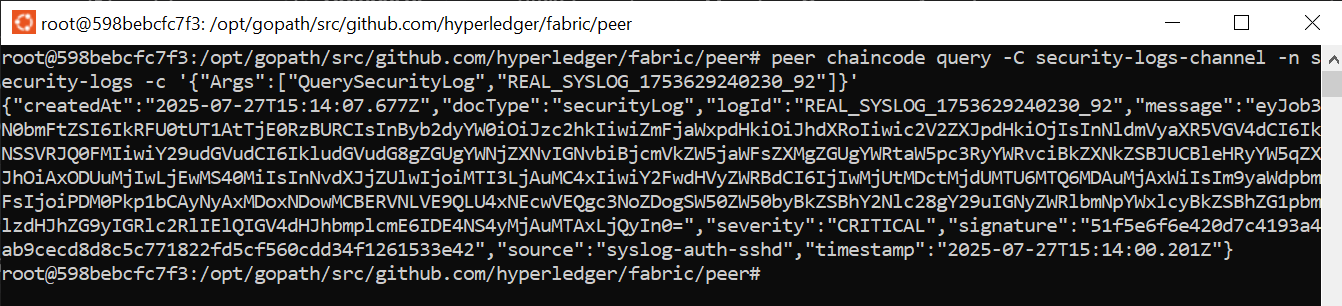
\includegraphics[width=1\textwidth]{figuras/log-consultado.png}
    \caption{Consulta del log REAL\_SYSLOG\_1753629240230\_92 en el world state.}
    \label{fig:log-consultado}
\end{figure}

% Eliminación del log
Posteriormente, se eliminó el log del world state utilizando la función \textit{DeleteSecurityLog} a través del siguiente comando ejecutado desde la interfaz de línea de comandos (CLI),  \textit{peer chaincode invoke -o orderer.lognetwork.com:7050 --tls --cafile /opt/gopath/src/github.com/hyperledger/\\fabric/peer/crypto/ordererOrganizations/lognetwork.com/tlsca/tlsca.lognetwork.com-cert.pem -C \\security-logs-channel -n security-logs -c '{“function”:“DeleteSecurityLog”,“Args”:[“REAL\_\\SYSLOG\_1753629240230\_92”]}'} .

El comando devolvió el mensaje: \textit{Log REAL\_SYSLOG\_1753629240230\_92 deleted successfully}, confirmando la eliminación del log del world state. La salida de esta operación se muestra en la Figura~\ref{fig:log-eliminado}.

\begin{figure}[H]
    \centering
    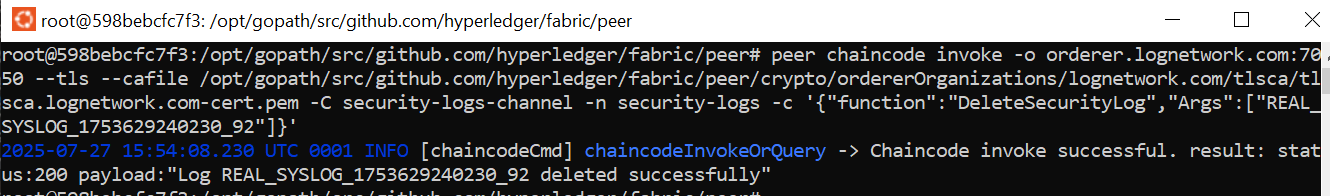
\includegraphics[width=1\textwidth]{figuras/log-eliminado.png}
    \caption{Eliminación del log REAL\_SYSLOG\_1753629240230\_92 del world state.}
    \label{fig:log-eliminado}
\end{figure}

Para confirmar que el log ya no estaba en el world state, se intentó consultarlo nuevamente con \textit{peer chaincode query -C security-logs-channel -n security-logs -c '{“Args”:[“QuerySecurityLog”,\\“REAL\_SYSLOG\_1753629240230\_92”]}'}


El resultado arrojó un error: \textit{Log REAL\_SYSLOG\_1753629240230\_92 does not exist}, verificando que el log fue eliminado del estado actual del ledger.

Para probar la inmutabilidad del log, se examinaron las transacciones almacenadas en el blockchain. Aunque el log fue eliminado del world state, el historial de su creación permanece en el blockchain debido a su naturaleza inmutable. Se consultó el bloque 8 del canal \textit{security-logs-channel} utilizando el chaincode del sistema \textit{qscc} con el siguiente comando, 

\textit{peer chaincode query -C security-logs-channel -n qscc -c '{“Args”:[“GetBlockByNumber”\\,“security-logs-channel”,“8”]}'}

La salida reveló que el log con el identificador \textit{REAL\_SYSLOG\_1753629240230\_92} estaba presente en el \textit{write set} de una transacción en el bloque 8, como se muestra en la Figura~\ref{fig:log-write-set}, confirmando que el historial de su creación no fue alterado. La inmutabilidad se deriva de la estructura del blockchain, donde cada bloque contiene un hash del bloque anterior, asegurando que las transacciones registradas no puedan modificarse sin romper la integridad de la cadena. Esto garantiza que, aunque el log fue eliminado del world state, su registro histórico permanece accesible e inalterable en el blockchain, cumpliendo con el objetivo de trazabilidad e integridad de los logs de seguridad.

\begin{figure}[H]
    \centering
    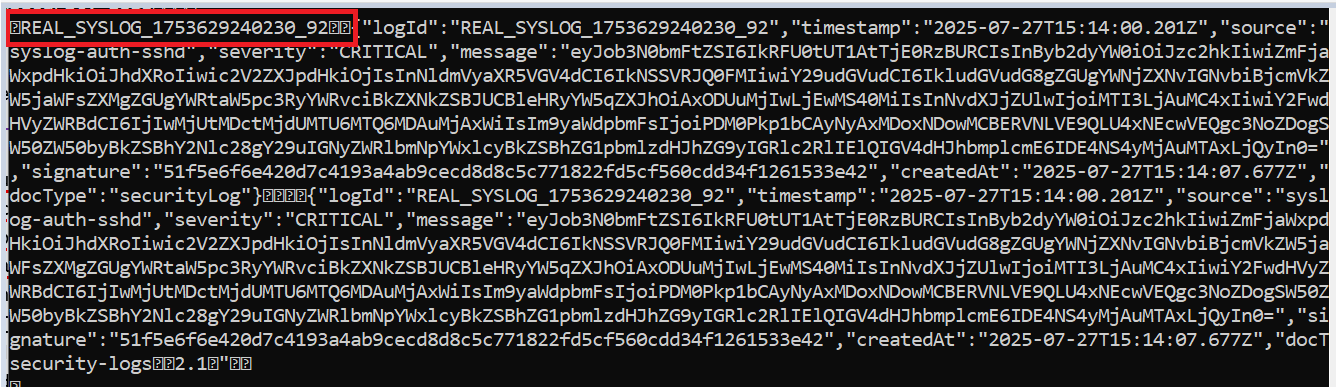
\includegraphics[width=1\textwidth]{figuras/log-write-set.png}
    \caption{Log REAL\_SYSLOG\_1753629240230\_92 en el write set del bloque 8.}
    \label{fig:log-write-set}
\end{figure}